\chapter{Grundlagen}
\label{cha:grundlagen}

Dieses Kapitel beschäftigt sich mit den für das Thema essentiellen Grundlagen. Darunter fallen neben der allgemeinen Funktion von Docker und Kubernetes sowie der Unterschiede zu virtuellen Maschinen auch Grundlagen zur persistenten Speicherung von Daten.

\section{Persistente Datenspeicherung}
\label{sec:persitenz}
Für den Betrieb von Anwendungen ist es wichtig, dass der Zustand und die generierten Daten der Anwendung langfristig gespeichert werden. Neben der Hardware, welche physisch für das Speichern der Daten zuständig ist, agiert die Software als Schnittstelle zwischen der Anwendung und den Datenträgern. Dabei bieten verschiedene Konzepte dieser Software unterschiedliche Vor- und Nachteile, so dass sie für verschiedene Anwendungsfälle geeignet sind.


\subsection{Die Herausforderung der Datenspeicherung}
Das persistente Speichern ist eine Herausforderung, welche bereits mit der Sicherstellung der Datensicherheit, also der Vertraulichkeit, der Integrität und der Verfügbarkeit von Daten anfängt. Darüber hinaus benötigen Anwendungen in modernen Infrastrukturen für die Reaktion auf unvorhersehbare Ereignisse wie sich schnell verändernde Anforderungen oder starke Beanspruchung der Systeme für die Datenspeicherung ein skalierbares und flexibles Konzept. Unabhängig von der Menge und der Größe der Daten wird eine Lösung benötigt, um von der Anwendung oder dem Nutzer generierte Daten wie Logdateien, Bilder, Videos usw. zu speichern. \medskip

Während bei monolithischen Anwendungen das Nutzen eines einzelnen Servers für die Speicherung von Daten oft ausreicht, benötigen verteilte Systeme und Cluster-Lösungen für ihr schnelllebiges und dynamisches Umfeld oft komplexere Lösungen. Dadurch entwickelten sich für die Datenspeicherung in diesen modernen Infrastrukturen verschiedene Möglichkeiten, die oft auf einem von drei grundlegenden Konzepten aufbauen.


\subsection{Konzepte der Datenspeicherung}
\subsubsection{File-Storage}
Ein File-Storage System speichert Daten in einer hierarchischen Struktur. Die Struktur wird ausgehend von einem Root-Verzeichnis mithilfe von Verzeichnissen aufgebaut. Um auf Dateien zuzugreifen, wird dabei aus den Dateinamen und den Verzeichnissen ein Pfad gebaut. Auf die physische Ebene eines Datenspeichers wird eine virtuelle Ebene, ein Dateisystem, aufgesetzt. Dabei gibt es viele verschiedene Dateisysteme, welche unterschiedliche Spezifikationen haben, und dadurch für verschiedene Anwendungsfälle geeignet sind.
Durch die zusätzliche Ebene bietet dieses Konzept eine höhere Latenz als zum Beispiel Block-Storage. Daten, welche gespeichert werden, enthalten einige Metadaten wie Zeit und Datum der Erstellung oder auch die Größe der Datei.
Der Speicher wird auf der Ebene des Dateisystems eingebunden und benötigt dabei bei den gängigen Betriebssystemen keine zusätzliche Software. Ein File-Storage kann durch die Nutzung von zusätzlichen Anwendungen um Funktionen wie Kompression der Daten oder das Erstellen von Sicherungen erweitert werden.
%zB Nas (smb/nfs), limited scale out, hight trhoughput, cost lower than block, komplex at scale, file type managment

\subsubsection{Block-Storage}
Bei einem Block-Storage werden Daten in gleichgroßen Blöcken gespeichert. Dabei enthält ein Block neben einer eindeutigen ID, um ihn zu identifizieren, keine zusätzlichen Metadaten. Werden Metadaten benötigt, müssen Daten auf Anwendungsebene mit diesen versehen werden. Um eine Datei zu modifizieren, müssen nur die veränderten Blöcke der Datei bearbeitet werden, ohne dabei den gesamten Block neu zu schreiben. Durch seine Struktur bietet ein Block-Storage eine niedrigere Latenz als ein File-Storage oder Objekt Storage. Dadurch eignet sich diese Art von Speicher gut für Transaktionsdaten sowie Daten die häufig geändert werden. 
Für die Verwaltung der Blöcke wird ein Controller benötigt, welcher Schreib- und Lesevorgänge auf die Blöcke ausführt.
%Complex at Scale, gut für Datenbanken, Controller verwaltet Blöcke, Latenz steigt, wenn Hardware weiter auseinander

\subsubsection{Object-Storage}
Ein Object-Storage System speichert Daten als sogenannte Objekte. Ein Objekt kann dabei eine variable Größe haben und jegliche Art von Daten enthalten \cite{ Mesnier2003StorageStorage}. Dabei ist es möglich, die Datei, neben der für die Identifizierung genutzten ID, mit benutzerdefinierten Metadaten zu versehen. So lassen sich auch für jedes Objekt individuell Sicherheits- oder Zugriffsrichtlinien festlegen \cite{ Mesnier2003StorageStorage}. Um eine Datei zu ändern, muss das komplette Objekt geladen und anschließend die veränderte Version neu gespeichert werden. Dadurch eignet sich diese Art von Speicher für statische Daten, welche zum Beispiel über eine \ac{HTTP} oder \ac{HTTPS} Schnittstelle abgerufen werden können. Dadurch bietet Objektspeicher eine sichere und plattformunabhängige Schnittstelle \cite{ Mesnier2003StorageStorage}. Um einen Objektspeicher mit einem herkömmlichen Protokoll einzubinden, wird eine zusätzliche Software benötigt.
Ein weiterer Vorteil von Object-Storage ist seine Ausfallsicherheit und Robustheit. Daten können über mehrere Server redundant gehalten werden und stehen so auch nach einem Ausfall eines Servers zur Verfügung.
% Versionierung möglich, einfache moven von Daten, hohe latenz, hoher durchsatz, prüfsummen möglich, zugriffmanament durch dateiowner
%Trennung von metadaten und Datne
% \cite{Zhou2012OptimizeStrategy}
%Distributed file systems have higher security, scalability and I/O efficiency.
%Block level cloud storage provides users with raw block device, on which users can create their own file system and database.


\section{Docker}
\label{sec:Docker}
Docker ist eine Open-Source Anwendung, welche es ermöglicht, Container zu erzeugen, auszuliefern und bereitzustellen. Container enthalten Anwendungen sowie alle Abhängigkeiten und Ressourcen die zur Laufzeit benötigt werden. Dabei bietet Docker selbst auch alle notwendigen Tools, um die Container zu verwalten. Docker erlaubt es, Anwendungen in einem Container zu starten und isoliert voneinander auf demselben Hostsystem ohne Hypervisor mit Hilfe der Docker-Engine (siehe \ref{subsec:dockerengine}) zu betreiben \cite{DBLP:journals/corr/Bui15,Soltesz2007Container-basedHypervisors}. Dabei wird beim Starten eines Containers kein Kernel geladen, sondern der Kernel des Hosts mitgenutzt.
Um die Anwendungen zu isolieren, werden im Linux Kernel integrierte Funktionen wie Cgroups und Namespaces eingesetzt \cite{Anderson2015Docker}. Durch die Isolation wird garantiert, dass ein Prozess innerhalb eines Containers keinen Zugriff auf Informationen über Prozesse oder die Nutzung von Ressourcen des Systems hat.
Durch die Auslieferung der Software mit allen Abhängigkeiten als Container ist sie plattform- und betriebssystemunabhängig. Die einzige Voraussetzung ist somit eine Plattform, welche Docker unterstützt.
Entwicklern ermöglicht ein sogenanntes Dockerfile (siehe \ref{subsec:dockerfile}), den Container sowie seine Infrastruktur zu konfigurieren.
%  Um Container zu starten, setzt Docker seit Version 0.9 statt der im Linux Kernel seit 2009 integrierten Linux-Container-Bibliothek (LXC) eine eigene Bibliothek namens libcontainer ein.
% Mehr zu Kernel Mapping

\subsection{Docker Engine}
\label{subsec:dockerengine}
Im Mittelpunkt steht die Docker Engine, welche für das Erzeugen und Bereitstellen der Container verantwortlich ist. Die Docker Engine ist eine, auf der Client-Server Architektur basierende, Applikation, welche aus drei Komponenten besteht \cite{doc:overview}.

\subsubsection{Docker Daemon}
\label{subsubsec:dockerdeamon}
Der Docker Daemon (dockerd) ist ein Prozess, der verantwortlich dafür ist, Anfragen über die API zu verarbeiten. Er läuft als root auf dem System. Eine weitere seiner Aufgaben ist die Verwaltung von Docker Objekten wie Containern und Images.
% Jemand mit Kontrolle über den dockerd prozess kann privilegierte Container starten die root einbinden können \cite{Grattafiori2016UnderstandingBy}

\subsubsection{Rest API}
\label{subsubsec:dockerapi}
Die \ac{REST} \ac{API}, welches vom Docker Daemon zur Verfügung gestellt wird, empfängt Kommandos vom Docker Client für die weitere Verarbeitung.

\subsubsection{Docker Client}
\label{subsubsec:dockerclient}
Der Docker Client ermöglicht es über ein \ac{CLI} und den \textit{docker} Befehl, mit dem Docker Daemon zu kommunizieren. Sobald ein Befehl über das \ac{CLI} ausgeführt wird, wird dieser vom Docker Daemon verarbeitet. Der Docker Client und der Docker Daemon müssen nicht auf demselben Host laufen.

\subsection{Dockerfile}
\label{subsec:dockerfile}
Das Dockerfile ist eine Textdatei, welche die Instruktionen für den Bau eines Docker Images enthält. Jede neue Zeile stellt eine neue Instruktion dar und erzeugt, außer bei wenigen Ausnahmen, eine neue Schicht auf dem stapelbaren Dateisystem des Images. Die erstellten Schichten werden zwischengespeichert, so dass bei einer Änderung des Dockerfiles nur die geänderte Schicht neu erstellt wird \cite{doc:overview}. Für das Interpretieren der Schritte und das Bauen des Images ist die Docker Engine zuständig. Typischerweise enthält ein Dockerfile Instruktionen wie FROM, um das Betriebssystem, welches als Basis dient, auszuwählen; RUN, um Befehle in dem Image auszuführen; VOLUME, um Datenträger einzubinden; EXPOSE, um Ports freizugeben und CMD, um den initialen Befehl des Containers festzulegen \cite{Grattafiori2016UnderstandingBy}.
\lstset{language=Dockerfile}
\begin{lstlisting}[frame=hlrtb, caption={Beispiel: Dockerfile} ,backgroundcolor=\color{white}, label={lst:DockerfileSample}]
FROM python:2

WORKDIR /usr/src/app

COPY . .

RUN pip install requests requests-toolbelt psycopg2

CMD ["python", "./application.py"]
\end{lstlisting}
Listing \ref{lst:DockerfileSample} zeigt ein beispielhaftes Dockerfile, um eine Python\footnote{\label{foot:python}Universelle Programmiersprache} Anwendung auszuführen. Als Basis wird hier das offizielle Python Image mit dem Tag \textit{2} gewählt. Danach wird das Arbeitsverzeichnis festgelegt und alle benötigten Dateien kopiert. Anschließend wird ein Befehl ausgeführt, der die für die Anwendung nötigen Pakete installiert und die Python Anwendung startet.

\subsection{Docker-Container und Docker-Images}
\label{subsec:dockerconimage}
Ein Docker-Image ist eine aus einem Dockerfile generierte, schichtweise aufgebaute Vorlage für Docker-Container. In dieser Read-Only Vorlage sind alle für das Erzeugen einer Container-Instanz benötigten Daten und Abhängigkeiten enthalten.

Ein Docker-Container stellt eine von einem Image ausgeführte Instanz dar. Aus einem Image können unbegrenzt viele Instanzen gestartet werden. Gestartete Container werden von dem Docker Client verwaltet und können so in unterschiedliche Zustände versetzt werden.
%states wie created, running, paused stopped, wichtigste

%\subsection{Vergleich virtuelle Maschinen mit Containern}
%\label{subsec:vmvsdocker}
%Obwohl es sich sowohl bei Containern als auch bei virtuellen Maschinen (VMs) um Techniken für die Virtualisierung handelt und beide oft verglichen werden unterscheiden sich die darunter liegende Architektur und die Einsatzmöglichkeiten. Beide Techniken schaffen eine virtuelle Umgebung für das Ausführen von Software. Bei einer VM wird im Gegensatz zu einem Container ein komplettes System, mittels eines Hypervisors, gestartet (vergleiche Abbildung \ref{fig:vmvsdocker}). Während der Unterschied zwischen Docker und einem nativen System in CPU-Geschwindigkeit und beim zufälligen Lesen von der Festplatte vernachlässigbar sind, sind virtuelle Maschinen dagegen fast immer langsamer \cite{Felter2015AnContainers}. Auch erhöht das Starten eines kompletten Systems den Speicherbedarf und verlängert die Zeit, die das System zum Starten benötigt.
%\begin{figure}[htb]
%\centering
%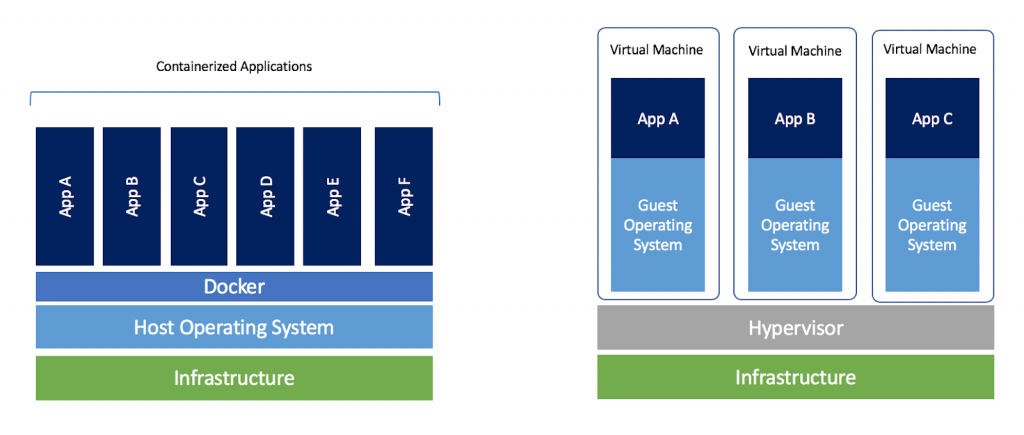
\includegraphics[width=1\textwidth,angle=0]{gfx/vmvsdocker2}
%\caption[Vergleich von Containern und virtuellen Maschinen]{Vergleich von Containern und virtuellen Maschinen % \cite{docker:vmvsdocker}}
%\label{fig:vmvsdocker}
%\end{figure}
%Gemeinsamkeiten finden sich darin, dass beide Technologien eine isolierte Umgebung für das Ausführen von Anwendungen bieten und dass sich sowohl VMs als auch Container aufgrund ihrer Beschaffenheit schnell und ohne Probleme zwischen verschiedenen Hosts umziehen lassen. Auch die Möglichkeit die Ressourcen für die Anwendung zu limitieren wird von beiden Technologien unterstützt.

\section{Kubernetes}
\label{sec:kube}
Kubernetes (griech. für Steuermann) ist eine von Google entworfene Plattform für das automatisierte Verwalten, Skalieren und Bereitstellen von Anwendungen in Containern. Google verwendet schon seit mehr als zehn Jahren Container in seinen Datencentern \cite{Burns2016BorgKubernetes}. Für die Verwaltung dieser wurde vorher die eigens entwickelte Plattform Borg und Omega genutzt. Als auch viele andere Entwickler begannen, sich für Linux-Container zu interessieren, wurde Kubernetes entwickelt \cite{Burns2016BorgKubernetes}. \medskip

Seit 2014 ist das System Open-Source und wird aktuell von der \ac{CNCF} gepflegt. Eine aktuelle Umfrage der \ac{CNCF} zeigt, dass Kubernetes zurzeit die führende Plattform ist und seine Konkurrenten wie Docker Swarm überholt hat \cite{kube:survey}. Ein Unterschied gegenüber anderen Lösungen ist, dass Kubernetes neben Docker auch andere Software für Container einsetzen kann, auf die in dieser Arbeit allerdings nicht weiter eingegangen wird.

\subsection{Kubernetes Architektur}
Ein Kubernetes Cluster besteht aus zwei Komponenten, welche sich in einer sogenannten Master-Slave-Architektur befinden. Die Architektur besteht aus einem Master, welcher aus einem oder mehreren Servern bestehen kann, und den von ihm verwalteten Slaves, in Kubernetes Nodes genannt (Abbildung \ref{fig:kubearchitektur}). Die Komponenten des Clusters können dabei sowohl lokal, auf physischen Servern oder virtuellen Maschinen als auch online auf Infrastruktur von Cloud-Computing Anbietern laufen.
\begin{figure}[htb]
\centering
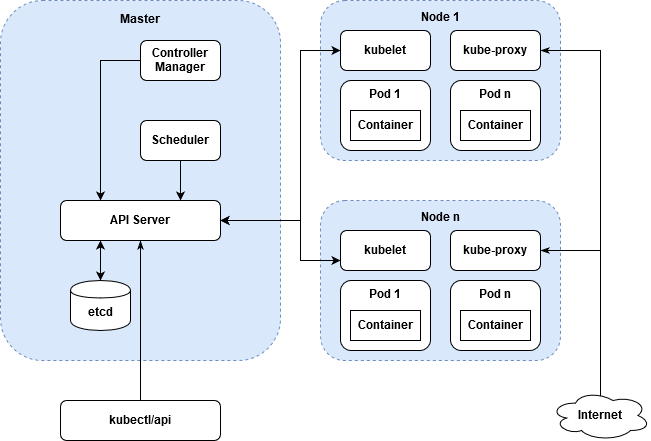
\includegraphics[width=0.8\textwidth,angle=0]{gfx/Kubernetes_Architektur}
\caption[Kubernetes Architektur]{Kubernetes Architektur}
\label{fig:kubearchitektur}
\end{figure}

\subsection{Master Node}
\label{masternode}
Der Master ist verantwortlich für die Verwaltung der Nodes im Cluster. Er leitet die Befehle vom Nutzer an die Nodes weiter. Er enthält mehrere für das Cluster wichtige Komponenten (vergleiche Abbildung \ref{fig:kubearchitektur}). Die Verwendung von mehreren Mastern ermöglicht es, ein hochverfügbares Cluster zu planen \cite[][]{9781788994729}. 

\subsubsection{API}
Der \textit{kube-apiserver} stellt die \ac{API} zur Verfügung, über die jegliche Kommunikation abläuft. Befehle, die der API Server über die Rest-Schnittstelle oder das \ac{CLI} erhält, verarbeitet er und reicht sie weiter \cite{Rensin2015Kubernetes43826}. Über die API ist es möglich, Kubernetes Objekte zu erstellen, zu bearbeiten und zu löschen.

\subsubsection{Controller Manager}
Auf dem \textit{kube-controller-manager} laufen die Controller. Auch wenn jeder Controller ein eigener Prozess sein könnte, werden sie, um die Komplexität zu reduzieren, in einem einzigen Prozess ausgeführt \cite{kube:components}. Dieser läuft auf dem Master und überwacht den Status des Clusters über die API. Verändert sich der gewünschte Status des Clusters, führen sie die nötigen Operationen aus, um das Cluster in den gewollten Status zu versetzen. Ein Beispiel hierfür wäre, wenn die Anzahl der geforderten Replicas nicht der Anzahl der existierenden entspricht. In diesem Fall würden neue Replicas gestartet werden. Der Controller Manager enthält unter anderem folgende Controller:
\begin{description}
\item[Replication Controller]
Der \textit{Replication Controller} ist dafür verantwortlich, die richtige Anzahl an Pods, welche eine logische Gruppe aus einem oder mehreren Containern darstellt (siehe \ref{kube:pod}), für jedes Replication Controller API Objekt beizubehalten.
\item[Endpoint Controller]
Erzeugt Endpoint Objekte, welche für die Verbindung von Services und Pods genutzt werden.
\item[Node Controller]
Bei dem Node Controller handelt es sich um einen Controller, welcher die Verfügbarkeit der Nodes im Clusters überwacht. Er reagiert, sobald ein Node nicht mehr verfügbar ist.
\item[Service Account \& Token Controller]
Dieser Controller er\-zeugt die Standard Accounts und verwaltet die Access Tokens \cite{kube:components}.
\end{description}

\subsubsection{Scheduler}
\label{kube:scheduler}
Um eine gleichmäßige Auslastung der Nodes zu gewährleisten, verteilt der Scheduler die Pods auf die Nodes. Dabei werden verschiedene Faktoren, wie die benötigten Ressourcen für die Anwendung und die Verfügbarkeit von Ressourcen auf dem Node bei der Auswahl der Nodes berücksichtigt. Abhängig vom Zustand des Clusters kann es auch vorkommen, dass Pods von einem Node auf einen anderen verschoben werden \cite{kube:components}.

\subsubsection{etcd}
Etcd\footnote{https://coreos.com/etcd/} ist ein leichtgewichtiger, verteilter Key-Value-Store, der die Konfiguration des Clusters sowie Informationen zu dessen Zustand speichert. Andere Komponenten des Clusters können über REST auf ihn zugreifen \cite[][]{9781788994729}. 

\subsubsection{Add-ons}
Bei Add-ons handelt es sich um Pods oder Services, welche die Funktionalität von Kubernetes erweitern. Ein Beispiel für ein Add-on ist das Web UI (Dashboard) für das Verwalten des Clusters und der Anwendungen, die dort laufen.
% raft consensus algortihm für HA \cite{Ongaro2014InVersion}

\subsection{Worker Node}
\label{workernode}
Sobald eine Anwendung im Cluster gestartet wird, werden die benötigten Pods auf den Nodes verteilt. Die Nodes stellen die Laufzeitumgebung für die Pods zur Verfügung. Jeder Node nutzt dabei dieselben Komponenten \cite{kube:components}. Die zwei wichtigsten Komponenten sind der Kube-Proxy und der kubelet \cite[][]{9781788994729}. 

\subsubsection{kubelet}
Der kubelet verwaltet die Pods und Container auf den Nodes. Er antwortet auf die Befehle vom Master und setzt diese um. Typische Befehle sind zum Beispiel das Erstellen, Überwachen und Zerstören von Containern auf dem Node \cite{Rensin2015Kubernetes43826}.
Eine weitere Aufgabe ist, den Status der Nodes an den Master zu melden.
% abgleich über endpoint/file path oder podscpec (yaml-&gt; updates

\subsubsection{Kube-Proxy}
Beim Kube-Proxy handelt es sich um einen Netzwerk Proxy, der Container und Service (siehe \ref{kube:service}) verbindet. Zusätzlich bietet er eine Lastverteilung. Der Proxy selbst unterstützt kein http, aber beherrscht dafür TCP und UDP Weiterleitung oder Round Robin für eine Lastverteilung.

\subsection{Pod}
\label{kube:pod}
Ein Pod ist die kleinste ausführbare Einheit in einem Kubernetes Cluster und repräsentiert eine laufende Anwendung. Innerhalb eines Pods ist es möglich, einen oder mehrere Container zu starten, welche miteinander gekoppelt sind. Diese teilen sich die Ressourcen wie Speicher, die IP-Adresse im Cluster oder das Netzwerk. Daher ist es Containern in einem Pod möglich, über \textit{localhost}\footnote{\label{foot:localhost}Standardisierter Domainname des aktuellen Computers} miteinander zu kommunizieren. Container in einem Pod werden beim Ausführen nicht über mehrere Nodes verteilt, sondern immer als eine Einheit auf einem Node ausgeführt. Der Node wird dabei durch den \textit{Scheduler} (siehe \ref{kube:scheduler}) anhand der Auslastung der Nodes und der vom Pods angeforderten Ressourcen gewählt.  \medskip

Wird eine Anwendung horizontal skaliert\footnote{\label{foot:scaleout}Erweitern der Kapazität durch zusätzliche Hard- oder Software}, startet ein zusätzlicher Pod, welcher eine eigenständige Instanz darstellt. Kubernetes empfiehlt, keine Pod Objekte von Hand zu erzeugen, und stattdessen ein Deployment (siehe \ref{kube:deployment}) oder für zustandsbehaftete Anwendungen ein StatefulSet (siehe \ref{kube:statefulset}) einzusetzen \cite{kube:pod2}. Ein manuell erzeugter Pod ist im Gegensatz zu von Controllern erzeugten und verwaltenden Pods nicht auf Beständigkeit ausgelegt und würde einen Absturz oder Fehler eines Nodes nicht überstehen.

\subsection{Services}
\label{kube:service}
Ein Service sorgt dafür, dass Pods für den Nutzer erreichbar sind. Ein Service ist ein REST API Objekt und bekommt eine IP-Adresse zugeteilt. Auch jeder Pod im Cluster hat seine eigene IP-Adresse, doch kann es passieren, dass sich ein Pod zum Beispiel durch den Replica Controller ändert. Dadurch würde der Pod eine neue Adresse zugeteilt bekommen. Um dies übersichtlicher zu gestalten und für den Nutzer zu vereinfachen, fügen Services eine zusätzliche Abstraktionsebene hinzu. Ein Service beschreibt dabei eine Regel, wie ein Pod erreicht werden kann. \medskip

Auf welche Pods ein Service weiterleitet, wird meistens über einen Label Selector festgelegt. Ein Label ist ein Key-Value Paar, welches einem Kubernetes Objekt wie einem Pod zugeordnet wird und selbst festgelegt werden kann. Über das Label ist so eine Identifikation des Objektes möglich.

\lstset{language=yaml}
\begin{lstlisting}[frame=hlrtb, caption={Beispiel: Kubernetes Service} ,backgroundcolor=\color{white}, label={lst:kubeservice}]
kind: Service
apiVersion: v1
metadata:
  name: app-service
spec:
  selector:
    app: App
  ports:
  - protocol: TCP
    port: 80
    targetPort: 8080
\end{lstlisting}
In dem Beispiel in Listing \ref{lst:kubeservice} wird ein Kubernetes Service Objekt erzeugt, welches den Namen \textit{app-service} hat. Der Service hat als Ziel Port 8080 bei jedem Pod mit dem Label \textit{App}. Das Ergebnis der Suche nach Pods mit dem festgelegten Label wird in ein Endpoint Objekt gespeichert. Zusätzlich bekommt der Service auch noch eine IP-Adresse im Cluster. Neben Services, welche als Proxy oder Loadbalancer agieren, gibt es in Kubernetes auch noch \textit{Headless Services}. Diese bieten die Möglichkeit, einen Pod direkt anzusprechen, und werden zum Beispiel für ein StatefulSet zwingend benötigt (siehe \ref{kube:statefulset}).
% clusterIP: None # erwähnen?

\subsection{Namespace}
Ein Namespace kann dafür genutzt werden, um verschiedene Bereiche auf dem Cluster, für verschiedene Projekte oder Teams abzugrenzen. Zur Identifizierung erhält der Namespace einen eindeutigen Namen. Durch Namespaces ist es ebenfalls möglich, Ressourcen zu limitieren.

\subsection{Ingresses}
Mit einem Ingress bietet Kubernetes eine einfache Möglichkeit, Zugriff auf Ressourcen des Clusters von außerhalb zu gewähren. Ein Kubernetes Cluster ist ein eigenes Netzwerk und isoliert grundsätzlich vor dem Zugriff von außen. In dem Ingress Objekt werden Regeln für das Routing über \ac{HTTP} oder \ac{HTTPS} von außerhalb sowie für die Konfiguration des Ingress gespeichert. Zusätzlich bietet er Optionen für Lastverteilung und SSL Termination. \medskip

Für den Ingress kann verschiedene Software benutzt werden. Im Kubernetes Projekt wird ein Nginx\footnote{\label{foot:nginx}Ein Open-Source Webserver, der auch als Reverse-Proxy genutzt werden kann} Ingress Controller und ein \ac{GCE} Ingress Controller unterstützt und gewartet.
%

\subsection{Controller}
Die unterschiedlichen Controller bieten für das Verwalten der Pods verschiedene Funktionen, die sich für verschiedene Einsatzzwecke eignen. Ein Controller läuft dabei in einer Kontrollschleife, welche den Zustand der von ihm verwalteten Pods über die Kubernetes API überwacht. Sollte der gewünschte Zustand vom aktuellen abweichen, führt er die nötigen Schritte aus, um den Zustand zu ändern.

\subsubsection{ReplicaSet \& ReplicationController}
Ein ReplicationController oder ReplicaSet sorgt dafür, dass mehrere Instanzen eines Pods existieren. Falls die Anzahl der angeforderten Replicas sich ändern sollte, sorgt der Controller dafür, dass weitere Replicas erzeugt oder entfernt werden. Durch diese Funktion lassen sich große Lasten verarbeiten oder eine höhere Verfügbarkeit erreichen. Eine Replica ist dabei eine Kopie eines Pods. Um die Anzahl der Replicas oder die Pods zu konfigurieren, wird ein sogenanntes Pod Template verwendet \cite{Rensin2015Kubernetes43826}. Trotz des Namens ist dieser Controller auch für einzelne Pods ohne Replicas sinnvoll, da er die Anzahl der Pods überwacht und so auf mögliche Abstürze reagiert.
Der bisher einzige Unterschied zwischen einem ReplicationController und dem neueren ReplicaSet ist die Art, wie sie Pods auswählen. Wird ein Controller entfernt bleiben die von ihm verwalteten Pods enthalten.
% Während der ReplicationController einen \textit{Equality Based Selector} verwendet, nutzt das ReplicaSet einen \textit{Set-Based Selector}.

\subsubsection{Deployment}
\label{kube:deployment}
Ein Deployment ist ein, in 2016 mit der Kubernetes Version 1.2 veröffentlichter Controller, der die Funktionalität eines ReplicaSets erweitert \cite[][]{9781788994729}. Für Pods die im Pod Template beschrieben sind, wird ein ReplicaSet erzeugt. Durch die zusätzliche Abstraktionsebene setzt er einige Funktionen wie zum Beispiel \textit{Rolling Updates} um. Dabei wird ein zusätzliches ReplicaSet für die neue Version des Pods gestartet und die alte erst entfernt, wenn die neue einwandfrei läuft. Kommt es zu Fehlern, wird das Update nicht ausgeführt.
Das Pod Template beschreibt, wie auch bei den anderen Controllern, einen gewünschten Zustand, den das Deployment überwacht und herstellt. Sollte ein Pod unerwartet abstürzen, wird er auch hier neu gestartet. \medskip

Das Listing \ref{lst:kubedeployment} zeigt beispielhaft eine YAML-Datei, welche dafür genutzt wird, ein Deployment Objekt, welches einen Postgres Datenbank Pod enthält, zu erzeugen.  \medskip
\newpage

\lstset{language=yaml}
\begin{lstlisting}[frame=hlrtb, caption={Beispiel: Kubernetes Deployment} ,backgroundcolor=\color{white}, label={lst:kubedeployment}]
apiVersion: apps/v1
kind: Deployment
metadata:
  name: postgres-deployment
spec:
  selector:
    matchLabels:
    app: postgres
  replicas: 2
  template:
    metadata:
      labels:
        app: postgres
    spec:
      containers:
      - name: postgres
        image: postgres:9.6
        ports:
        - containerPort: 5432
\end{lstlisting}
%empohlener Kontroller, RelicaSet nur wenn Updates selber machen will oder garkeine Braucht.

\subsubsection{StatefulSet}
\label{kube:statefulset}
Das \textit{StatefulSet} eignet sich besonders für Anwendungen, deren Zustand bewahrt werden soll. Im Gegensatz zu einem Deployment sorgt es dafür, dass Pods eine einzigartige Bezeichnung bekommen, welche über die Laufzeit hinweg bestehen bleibt. Anhand dieser Bezeichnungen werden dem StatefulSet auch die Ressourcen zugeteilt. Wird ein Pod mit denselben Spezifikationen erneut gestartet, bekommt er vom Controller dieselbe Bezeichnung und die gleichen Ressourcen zugeteilt. Darüber hinaus bieten StatefulSets die Möglichkeit, Pods geordnet zu starten.
Auch der StatefulSet Controller, welcher seit Version 1.9 in einer stabilen Version verfügbar ist, versucht, wie die anderen Controller, einen gewünschten Zustand herzustellen. Sollte der Zustand nicht der gewünschte sein, werden die nötigen Schritte, um ihn zu ändern, eingeleitet. Zusätzlich benötigt ein \textit{StatefulSet}, im Gegensatz zu einem ReplicaSet oder einem Deployment, noch einen \textit{Headless Service} (siehe \ref{kube:service}) für die Identifizierung im Netzwerk.
Das Entfernen eines StatefulSet löscht nicht die mit den Pods verbunden Ressourcen. So kann für zustandsbehaftete Anwendungen die Datensicherheit garantiert werden.

\subsubsection{DaemonSet}
Der Daemonset Controller sorgt dafür, dass auf jedem Node oder einem Teil der Nodes des Clusters eine Instanz eines Pods läuft. Daher eignet sich dieser Controller besonders gut für Daemons oder Agents. Sollte ein Node vom Cluster entfernt oder zum Cluster hinzugefügt werden, kümmert sich der Controller darum, die Anzahl der Instanzen an die Anzahl der Nodes anzupassen.

\subsection{Helm}
Helm ist ein Werkzeug zum Verwalten von Anwendungen in Kubernetes. In sogenannten Helm Charts wird der Zustand von Anwendungen definiert. Die Verwendung von Helm vereinfacht sowohl die Installation als auch die Wartung der Anwendungen. Dabei ist es möglich, Objekte dynamisch zu definieren, oder Werte, ohne direktes Bearbeiten der Dateien, zu überschreiben. Dadurch ist es zum Beispiel ohne Aufwand möglich, eine andere Version eines Docker Images einzubinden. Wie auch Kubernetes wird Helm von der \ac{CNCF} verwaltet \cite{Helm}. Helm bietet einen offiziellen Katalog, der Anwendungen in stabilen Charts zur Verfügung stellt und standardmäßig installiert wird \cite{helm:github}. Diese können durch den \textit{helm install} Befehl installiert werden.

\subsubsection{Helm Charts}
\label{helm:chart}
Die sogenannten Helm Charts bestehen aus einem Verbund mehrerer Dateien, welche die Anwendung und ihren Zustand definieren. Dabei werden verschiedene Charts über die Verzeichnisstruktur abgegrenzt. Wichtige Dateien sind die \textit{Charts.yaml}, welche allgemeine Informationen über den Chart enthält, die \textit {requirements.yaml}, welche Informationen über Abhängigkeiten enthält und die \textit{values.yaml}, welche für die Konfiguration der den Variablen zugeordneten Werten genutzt wird.

\section{Persistenz in Kubernetes}
Für die persistente Speicherung von Daten kann in Kubernetes zwischen einer Vielzahl an Möglichkeiten gewählt werden. Durch die Verwendung von Volume Plugins ist es möglich, Volumes dynamisch erzeugen zu lassen oder sie bereits vorher für die Verwendung zu erzeugen. \medskip
\begin{figure}[htb]
\centering
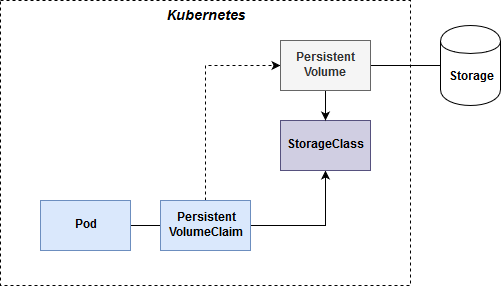
\includegraphics[width=0.8\textwidth,angle=0]{gfx/kubevolumelifecycle}
\caption{Zusammenhang Pod und Volume}
\label{fig:kubevolumelifecycle}
\end{figure}


Die Konfiguration des von Pods angeforderten Speichers geschieht direkt bei der Konfiguration des Pods über ein sogenanntes \ac{PVC}. Bei der statischen Bereitstellung von Volumes wird zunächst geprüft, ob ein \ac{PV} mit mindestens der geforderten Größe existiert, und das am besten passende eingebunden. Wird hier kein \ac{PV} gefunden und ist die dynamische Erstellung nicht konfiguriert, wird auf die Erzeugung eines Speichers gewartet \cite{kube:pv}. Die dynamische Methode bietet die Möglichkeit, das benötigte Volume durch das in der \ac{SC} Provisioner genannte Volume Plugin erzeugen zu lassen. \medskip

Die Abbildung \ref{fig:kubevolumelifecycle} zeigt den Ablauf der Erstellung eines \ac{PV}s. Fordert ein Pod durch eine \ac{PVC} Speicher an, so erstellt die \ac{SC} dynamisch ein \ac{PV}, welches der Konfiguration des \ac{PVC} entspricht.

\subsection{Persistent Volumes}
\label{kube:pv}
Ein PersistentVolume bietet in Kubernetes die Möglichkeit, Daten persistent zu speichern. So sind Daten erneut verfügbar sollte ein Pod aufgrund eines Fehlers neu gestartet werden. Die Verwendung von \ac{PV}s ermöglicht es, die Art und Weise wie der Speicher genutzt wird von der Bereitstellung abstrahiert zu betrachten. Für die Bereitstellung von \ac{PV}s gibt es zwei Möglichkeiten. Bei der statischen Provisionierung ist es nötig, dass alle \ac{PV}s manuell angelegt werden. Direkt nach dem Anlegen sind sie für die Nutzung verfügbar. Die zweite Möglichkeit ist das dynamische Provisionieren. Dabei wird ein neues Volume für die Anforderungen erzeugt. Dafür wird das \ac{PVC} des Pods betrachtet, in dem der angeforderte Speicher konfiguriert ist. Dort ist neben der Größe des Speichers und weiteren Einstellungen auch eine \ac{SC} definiert \cite[][]{9781788994729}. 

\subsection{Persistent Volume Claim}
\label{kube:pvc}
Durch ein \ac{PVC} ist es möglich, das gewünschte \ac{PV} näher zu spezifizieren. Es lässt sich bereits während der Erstellung des Pods konfigurieren. Dabei enthält ein \ac{PVC} Objekt einige Informationen wie einen Namen für die Identifikation, die Größe des benötigten Speichers und einige weitere Einstellungen für den Speicher (Listing \ref{lst:kubepvc}).  \medskip

Der Zugriffsmodus ist eine wichtige Einstellung, welche definiert, wie der Speicher eingebunden ist. Der Speicher kann nach Bedarf nur mit Leserechten oder mehrfach eingebunden werden. Dadurch lässt sich der Speicher unterschiedlichen Einsatzzwecken anpassen.
\begin{description}
\item[ReadWriteMany]
\ac{RWX} erlaubt es, den Speicher in einem oder mehreren Pods einzubinden. Dadurch ist es möglich, dass Pods über den Speicher Daten austauschen. Schreib- sowie Lesezugriff sind möglich.
\item[ReadWriteOnce]
\ac{RWO} erlaubt es, einen Speicher in genau einem Pod einzubinden. Schreib- sowie Lesezugriff sind möglich.
\item[ReadOnlyMany]
\ac{ROX} kann wie \ac{RWX} mehrfach eingebunden werden, allerdings sind nur Lesezugriffe möglich. Daher eignet es sich vorallem für statische Daten, die in mehreren Pods verfügbar sein sollen.
\end{description}
Die nächste wichtige Option ist die Wahl der \ac{SC}. Sie wird für die dynamische Erstellung von Speicher benötigt (siehe \ref{kube:sc}).
\lstset{language=yaml}
\begin{lstlisting}[frame=hlrtb, caption={Beispiel: Kubernetes PersistentVolumeClaim (PVC)} ,backgroundcolor=\color{white}, label={lst:kubepvc}]
kind: PersistentVolumeClaim
apiVersion: v1
metadata:
  name: claim
spec:
  accessModes:
  - ReadWriteOnce
  resources:
    requests:
      storage: 8Gi
  storageClassName: sc-name
\end{lstlisting}
Das Listing \ref{lst:kubepvc} zeigt eine beispielhafte Konfiguration eines \ac{PVC}. Dabei wird von der \ac{SC} \textit{sc-name} ein Speicher mit einer Kapazität von acht GB und dem Zugriffmodus \ac{RWO} angefordert.

\subsection{Storage Class}
\label{kube:sc}
Durch die Verwendung von mehreren \ac{SC}s ist es möglich, verschiedene Arten von Speicher anzubieten. So kann durch den Einsatz unterschiedlicher Technologien oder der Einbindung von unterschiedlicher Hardware auf unterschiedliche Anforderungen reagiert werden. \medskip

Es ist möglich, eine \ac{SC} als Standard zu benennen, welche immer wenn in einem \ac{PVC} keine \ac{SC} benannt wird genutzt wird.
Das \ac{SC} Objekt enthält Informationen wie das als Provisioner gewählte Volume-Plugin und Parameter, um ihn zu konfigurieren. Desweiteren lassen sich Regeln für eine erneute Beanspruchung von dynamisch erstellten Volumen oder zusätzliche Optionen für das Einbinden des Speichers konfigurieren. Mögliche Regeln für die erneute Beanspruchung sind Retain, Delete und Recyle.
\begin{description}
\item[Retain]
Retain bedeutet nach dem Löschen des \ac{PV} bleiben die Daten bestehen und müssen manuell auf dem System gelöscht werden. Durch ein erneutes Erstellen des dazugehörigen \ac{PV} lassen sich die Daten erneut nutzen.
\item[Delete]
Bei Delete werden durch das Löschen des dazugehörigen \ac{PV} die Daten auf dem System automatisch entfernt. Bei dynamisch erstellten \ac{PV}s werden die Regeln für eine erneute Beanspruchung der StorageClass verwendet. Falls in der StorageClass keine Regeln spezifiziert wurden, ist \textit{Delete} der Standardwert.
\item[Recycle]
Recycle ist eine veraltete Regel, welche durch das dynamische Provisionieren ersetzt wurde. Sie entfernt den Inhalt des eingebundenen \ac{PV}s. Dadurch ist es bereit, erneut eingebunden zu werden.
\end{description}
\lstset{language=yaml}
\begin{lstlisting}[frame=hlrtb, caption={Beispiel: Kubernetes StorageClass}
,backgroundcolor=\color{white}, label={lst:kubesc}]
kind: StorageClass
apiVersion: storage.k8s.io/v1
metadata:
  name: standard
provisioner: kubernetes.io/provisioner
reclaimPolicy: Retain
volumeBindingMode: Immediate
\end{lstlisting}
Das Listing \ref{lst:kubesc} zeigt beispielhaft die Erstellung einer \ac{SC} mit dem Namen \textit{standard}. Neben der Wahl des Provisioners \textit{kubernetes.io/provisioner} wird die Regel für die erneute Beanspruchung des Speichers auf \textit{Retain} gesetzt.

\subsection{Volume Plugin System}
Ohne Hilfe durch Tools müssten von Dritten erstellte Plugins fest in Kubernetes integriert und mit Kubernetes ausgeliefert werden. Um auch ohne diese Integration die Möglichkeit zu haben eigene Volume Plugins erstellen zu können, existieren derzeit zwei Möglichkeiten. Das seit Version 1.2 existierende Flex Volume, welches eine \ac{API} für externe Plugins bereitstellt, oder das seit Version 1.10 im Beta Status existierende \ac{CSI}.

\subsubsection{FlexVolume}
Bei FlexVolume handelt es sich um ein Tool, welches eine API für Volume Plugin von Dritten zur Verfügung stellt. Um die Speichertreiber zu nutzen, müssen die Nodes vorbereitet werden und die nötigen Daten auf das System kopiert werden. Dafür wird Zugriff auf alle Nodes des Clusters benötigt. Seit Version 1.8 erkennt FlexVolume, ohne einen Neustart der betroffenen Nodes, wenn neue Treiber hinzugefügt oder alte aktualisiert werden.

\subsubsection{Container Storage Interface}
Das \ac{CSI} ist eine Schnittstelle für Plattformen wie Kubernetes, um die Persistenzlösungen den Containern zugänglich zu machen. Es befand sich bis Version 1.12 im Beta Status und ist seit der Version 1.13 in einer stabilen Version verfügbar. \medskip

Eine Konfiguration des \ac{CSI} ist über Parameter möglich. Dort lassen sich der Treiber, der genutzt werden soll, die Art des Dateisystems und weitere Optionen konfigurieren.
